% -*- coding: utf-8; -*-

\chapter{Geração Semiautomática}
\label{gordon}

	Kindlmann e Durkin foram uns dos primeiros a gerar funções de transferência para visualizar as fronteiras de um volume de dados. Apesar de ter sido publicado há quase 20 anos e de possuir problemas na identificação de fronteiras em que a variação de seus valores se sobrepõem, seu trabalho ainda é o mais equilibrado no quesito \quote{Geração automática \textit{X} Controle do usuário}. Principalmente se analisado segundo a versão 1D de sua função de transferência.
	
	
	Como visto no Capítulo~\ref{related}, o trabalho de \textit{Kindlmann e Durkin}~\cite{gordon} é o que menos exige iteração do usuário para detectar fronteiras automaticamente e, ao mesmo tempo, permitindo que este possa controlar a função de transferência gerada.
	Faça uma apresentação do método....extende o trabalho relacionado + introdução e (talvez) emende nesse início de deteção de fronteira...(talvez não rs).
\section{Detecção de fronteiras}
\label{gordon.bound}
	\textit{Kindlmann e Durkin}~\cite{gordon} partem do princípio que toda fronteira é caracterizada por uma variação abrupta na intensidade de um material. Uma vez que também é assumido que os materiais são homogêneos, uma fronteira pode inicialmente ser modelada pela função degrau. No entanto, devido a uma limitação da aquisição de dados, as fronteiras são comumente borradas com uma resposta gaussiana na frequência. Por esse motivo, o comportamento de uma fronteira deve ser modelado como a convolução da função degrau com uma gaussiana. O resultado dessa convolução é a função \textit{erf()}, ou função \textit{erro}, ilustrada na Figura~\ref{fig:boundary_model}.
	
\begin{figure}[h]
	\centering
	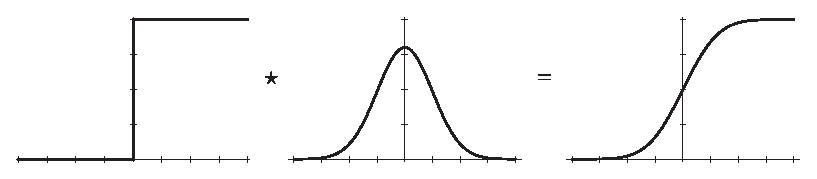
\includegraphics[width=1\textwidth]{images/g_boundary_model}
	\caption{Comportamento das funções degrau, gaussiana e erro, respectivamente.~\cite{gordon}.}
	\label{fig:boundary_model}
\end{figure}

	A função \textit{erf()} é uma função contínua cuja imagem varia de $-1$ a $1$. Como uma fronteira pode variar entre quaisquer dois valores escalares contidos no volume, a função $f(x)$ deve variar de $s_{min}$ a $s_{max}$ com o comportamento de \textit{erf()} para poder modelar corretamente uma fronteira. Assim, $f(x)$ é definida como a equação~\eqref{eq:boundary} abaixo:

\begin{equation} \label{eq:boundary}
	f(x) = s = s_{min} + (s_{max} - s_{min}) \frac{1 + erf(\frac{x}{\sigma\sqrt{2}})}{2}
\end{equation}
	
	A equação \eqref{eq1}...
    
\section{1d}
\label{gordon.1d}
	Texto...
    
\section{2d}
\label{gordon.2d}    
    Texto..
    
\section{Avaliação do método}
\label{gordon.aval}    
    Atacar treshold do gordon, apresentando minha solução. Mas sem criticar de forma negativa.
    
    Comentar 2ª derivada média.